\documentclass[fleqn]{jbook}
\usepackage{physpub}

\begin{document}

\begin{question}{専攻 問題4}{}

% Definition of local macros
\def\Po{\Atom{Po}{84}{212}}
\def\Au{\Atom{Au}{79}{197}}
\def\Pb{\Atom{Pb}{82}{208}}
\def\He{\Atom{He}{2}{4}$^{\rm 2+}$}
\def\Al{\Atom{A\ell}{13}{27}}
\def\A{$\alpha$}

真空箱の中に, \A 線源のポロニウム (\Po)、金 (\Au) の薄膜標的、スリット
、シリコン半導体検出器 (SSD) を模式図のように配置してラザフォード散乱
実験を行なった。\A 粒子の運動エネルギーは、$T_{\alpha}=9 \Unit{[MeV]}$
であった。簡単のために、標的の質量は \A 粒子の質量にくらべて十分に
大きく標的の反跳効果は無視できるものとする。なお、\A 粒子はヘリウムの
原子核であり {\He} である。また, 質量数 A の原子核の半径は、
$r = 1.2 \cdot A^{1/3} \Keta{-15} \Unit{[m]}$ で与えられる。
必要に応じて次の数値を参照せよ。
%
\begin{eqnarray*}
  && N_A(\mbox{アボガドロ数})=6\Keta{23}\Unit{[個/mol]},\hspace{10mm}% 
     \hbar c = 200 \Keta{-15}\Unit{[MeV \cdot m]},\hspace{10mm}%
     \frac{e^2}{4 \pi \varepsilon_0 \hbar c} = \frac{1}{137} \\
  &&   4^{\frac{1}{3}} = 1.6, \hspace{10mm}%
     197^{\frac{1}{3}} = 5.8, \hspace{10mm}%
     212^{\frac{1}{3}} = 6.0, \hspace{10mm}%
     208^{\frac{1}{3}} = 5.9
\end{eqnarray*}
%
\begin{center}
  \mbox{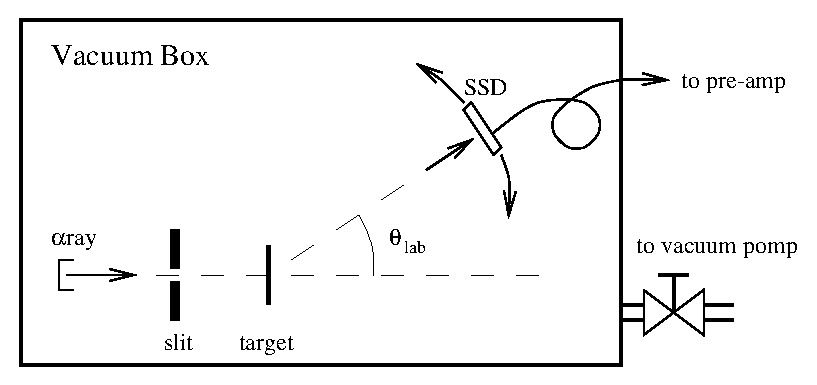
\includegraphics[clip]{1996phy4-1.eps}}
\end{center}


\begin{subquestions}
\SubQuestion 
  実験を真空中で行なう理由を1行以内で述べよ。

\SubQuestion
  \Po は、\A 崩壊を起こし 鉛 \Pb に変換する。鉛の核表面における
  \A 粒子に対するクーロン障壁の大きさを \Unit{[MeV]} 単位で求め、
  \A 崩壊のメカニズムを定性的に述べよ。

\SubQuestion
  \A 粒子が、前方(例えば $30\deg$)と後方(例えば $150\deg$)に散乱され
  たときのそれぞれの軌道を、衝突径数 $b$ や最近接距離$b_0$ などの
  大小関係が判るように、一つの図の中に描け。ただし、散乱過程は古典力学
  的に取り扱うことができ、古典的軌道を描くことができるとする。また、
  軌道と $b$ や $b_0$ の関係式や具体的な値を求める必要はなく、定性的な
  ことが判るように図示されていれば十分である。

\SubQuestion
  標的にスリットを通って入射する \A 粒子数を $I \Unit{[個/秒]}$、金の
  原子数を $N \Unit{[個/m^2]}$、検出器の立体角を
  $\IDelta \Omega \Unit{[sr]}$、微分散乱断面積を
  $(\tDeriver{\sigma}{\Omega})_R$ $\Unit{[m^2/sr]}$とする。

  \begin{subsubquestions}
  \SubSubQuestion 
    計数率 $Y$\Unit{[個/秒]}を求める式を書き下せ。
  \SubSubQuestion
    金薄膜の厚さは $1\Unit{[g/m^2]}$である。金の原子数を
    $\Unit{[m^{-2}]}$ 
    の単位で求めよ。
  \SubSubQuestion
    標的から検出器までの距離は $0.2 \Unit{[m]}$、また検出器の有感面積は
    $4 \Keta{-4} \Unit{[m^2]}$ であった。立体角を求めよ。
  \SubSubQuestion
    $I$ が $10^8 \Unit{[個/秒]}$のときに、散乱角度 $60\deg$ に散乱した
    \A 粒子を検出し、$1 \%$ の統計精度の個数になるまで計数したい。
    これに必要な測定時間をもとめよ。ただし \A 粒子の検出効率は $100\%$
    とする。ここで、点電荷 $Z_A$ によるラザフォード散乱は式
%
    \[ \Bigl(\Deriver{\sigma}{\Omega}\Bigr)_R %
       = \Bigl(\frac{2 Z_A e^2}{4 \pi \varepsilon_0}\Bigr)^2 %
         \frac{1}{T_{\alpha}^2 \cdot \sin^4{\theta/2}} \]
%
    で与えられる。
  \end{subsubquestions}

\SubQuestion
  金の原子は $79$ 個の電子を持っているが、この電子がラザフォード散乱の
  角度分布に与える影響を議論せよ。

\SubQuestion
  標的をアルミニウム (\Al) の薄膜に変えて測定を行ったところ 
  下図の結果を得た。ここで、横軸は散乱角度 ($\theta_{\rm lab}$)、
  縦軸はラザフォード比と呼ばれる量であり、測定で得た微分散乱断面積
  $(\tDeriver{\sigma}{\Omega})_{exp}$ をラザフォード
  散乱で予想される微分散乱断面積
  $(\tDeriver{\sigma}{\Omega})_{R}$ 
  で規格化したものである。  
  
  \begin{subsubquestions}
  \SubSubQuestion
    大きな散乱角度から小さな散乱角度に向かって測定を行ったところ、
    ラザフォード比の値がだんだんと$1$からずれて小さくなった。\\
    この原因として考えられることを、検出器の計数効率を考慮して
    簡潔に推論せよ。また、その様なことが起こらないようにする
    実験的工夫を述べよ。

  \SubSubQuestion
    最近接距離 $b_0$ が原子核の半径程度になると、原子核反応を
    引き起こす。図のなかのどこにその様なことが現れているか。
    簡潔に説明せよ。

  \end{subsubquestions}

  \begin{center}
    \mbox{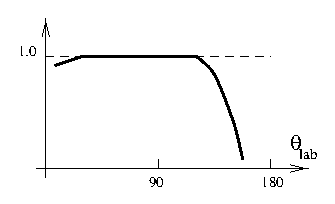
\includegraphics[clip]{1996phy4-2.eps}}
  \end{center}

\end{subquestions}
\end{question}
\begin{answer}{専攻 問題4}{}

% Definition of local macros
\def\Po{\Atom{Po}{84}{212}}
\def\Au{\Atom{Au}{79}{197}}
\def\Pb{\Atom{Pb}{82}{208}}
\def\He{\Atom{He}{2}{4}$^{\rm 2+}$}
\def\Al{\Atom{A\ell}{13}{27}}
\def\A{$\alpha$}


\begin{subanswers}
\SubAnswer
  空気のせいで \A 粒子のbeam 強度が落ちる。

\SubAnswer
  \Pb の核半径$r$は
  $ r = 1.2 \cdot 208^{1/3} \Keta{-15} \Unit{[m]}%
       = 7.08 \Keta{-15} \Unit{[m]} $。
  Coulomb potential は
%
  \[ \frac{e^2}{4\pi\varepsilon_0\hbar c} \hbar c%
     \frac{Z_\alpha Z_{\rm Pb}}{r}
   = \frac{1}{137} \times 200 \Keta{-15}
     \Unit{[MeV \cdot m]} \times
     \frac{2 \cdot 82}{7.08 \Keta{-15} \Unit{[m]}}%
   = 33.8 \Unit{[MeV]} \simeq 34 \Unit{[MeV]} \] 
%
%  つまり、$34\Unit{MeV}$ の Coulomb 障壁をトンネル効果\\
%  で通り抜けて、$9\Unit{MeV}$ だけ安定化するわけである
   \A 粒子内の4つの核子間の結合エネルギーの埋め合わ
   せとして得られる運動エネルギーにより、トンネル効果を\\
   起こして$34[\Unit{MeV}]$のCoulomb障壁を通り抜ける。\\
   透過後は$9[\Unit{MeV}]$の運動エネルギーを持つ。

\SubAnswer
  \parbox[t]{78mm}{
  $ b_0 (150\deg) < b_0 (30\deg)$であり、軌道は双曲線で対称で、\\
  衝突径数は保存される。右図の通りである。
  }\parbox[t]{80mm}{\vspace*{-20mm}
  \begin{center}
    \mbox{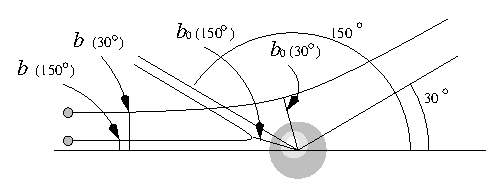
\includegraphics[clip]{1996phy4-3.eps}}
  \end{center}}
\vspace*{-8mm}
\SubAnswer
  \begin{subsubanswers}
  \SubSubAnswer
    スリットの断面積を$S\Unit{[m^2]}$と表せば、
    $\d{\sigma}\Unit{[m^2]}$\\
    の断面積内から来る粒子の流量は
    $I\d{\sigma}/S \Unit{[個/秒]}$である。それが一つの原子核により
    散乱されて$\d{\Omega}\Unit{[sr]}$の角度に広がる。
    他の$NS$個の原子核からの散乱もこの角度に入るため、流量は$NS$倍に
    なる。よって$ \IDelta \Omega \Unit{[sr]}$の角度に入る流量
    $Y\Unit{[個/秒]}$は
%
    \[ Y = \frac{I\d{\sigma}}{S} \cdot%
           NS \cdot \frac{\IDelta \Omega}{\d{\Omega}}
         = \Bigl(\Deriver{\sigma}{\Omega}\Bigr)_R%
           NI \IDelta \Omega \]
%

  \SubSubAnswer
    $6 \Keta{23} \Unit{[個]}$ が $197\Unit{[g]}$ にあるので、
    $1\Unit{[m^2]}$の$1\Unit{[g]}$ 中の個数、すなわち数密度$N$は
%
    \[ N = 6 \Keta{23}/197 = 3.05 \Keta{21} \Unit{[個/m^2]} \]
%

  \SubSubAnswer
    立体角とは、それが半径$1\Unit{[m]}$の球面上に張る面積である。
%
    \[ \IDelta \Omega% 
       = 4 \Keta{-4} \times (\frac{1}{0.2})^2 = 0.01 \Unit{[sr]} \]
%

  \SubSubAnswer
    \A 粒子の生成は確率的なので、その計測数 $C\Unit{[個]}$ 
    はポアッソン分布あるいはガウス分布となる。よってその標準偏差
    は $\sqrt{C}$ で与えられ、これが測定値の統計誤差となる。
    この誤差が$0.01$となるためには
%
    \[ \sqrt{C}/C = 0.01 \hspace{15mm}%
       \Yueni C = 10000\Unit{[個]} \]
%
    これだけの\A 粒子を測定しなければならない。\\
%
    次に散乱角度$60\deg$での計数率 $Y$ を計算する。与えられた
    ラザフォード散乱の公式より
%
    \[ \Bigl(\Deriver{\sigma}{\Omega}\Bigr)_R %
       = \Bigl( \frac{1}{137} \cdot 200\Keta{-15}\Unit{[MeV]} \cdot%
              2 \cdot 79 \Bigr)^2 %
         \frac{1}{ (9\Unit{[MeV]})^2 \cdot \sin^4{30\deg} }%
       = 1.05\Keta{-26}\Unit{[m^2/sr]} \]
%
    \[ Y = 1.05 \Keta{-26}\Unit{[m^2/sr]} \cdot%
           3.05 \Keta{21} \Unit{[個/m^2]} \cdot%
           10^8 \Unit{[個/秒]} \cdot%
           0.01 \Unit{[sr]}%
         = 32.0 \Unit{[個/秒]} \]
%
    \[ \Yueni t = \frac{C}{Y}%
                = \frac{10000\Unit{[個]}}{32.0 \Unit{[個/秒]}}%
                = 313 \Unit{[秒]} \]
%
    

%    \begin{tabular}{lcl}
%      \Yueni ~ $t$ & = & $10000 \cdot 
%                   \{ (\frac{1}{137} \cdot 200 \cdot 10^{-15}
%                      \cdot 2 \cdot 79 \cdot 2 )^2 
%                        \cdot 
%                        \frac{1}{9 \cdot 9 \cdot \sin^4 30 \deg}
%                        \cdot 1.18 \cdot 10^{20} \cdot 10^8 \cdot 0.01
%                   \}^{-1}$ \\
%                         
%    & = & $1941 \Unit{[秒]}$
%
%   \end{tabular}  
%
%   \Yueni 約32分 
  \end{subsubanswers}


\SubAnswer
  小角度(最近接距離大)のとき、電子の遮蔽効果により原子核の電荷
  $eZ$ が小さく感じられる。
  $Y \propto (\tDeriver{\sigma}{\Omega}) \propto Z^2$ なので
  すなわち、$Y$ が Rutherford 式からの予想に比べて小さくなる。

\SubAnswer
  \begin{subsubanswers}
  \SubSubAnswer
    問題としている小角度では、$(\tDeriver{\sigma}{\Omega})$
    が非常に大きくなるので、 $Y$ も大きくなる。
    これにより検出器の dead time が大きくなって、$Y$が小さく
    観測されるのである。この対策として考えられる方法として、
     時間分解能のいいmoduleを使用する、
    入射 beam 強度を落して、測定時間を増やして、calibration する
    ($Y \rightarrow Y \cdot \frac{\mbox{real time}}{\mbox{live time}}$
    にかえて plot)、などが考えられる。

  \SubSubAnswer
    大角度散乱で$Y$が小さくなっている。
    これは最近接距離が核の半径と同程度になり、
    原子核反応が起こっていることを示す。
    (\Au では核のポテンシャルが強力すぎる。\Al では弱いので、
    $9 \Unit{[MeV]}$の \A でも十分近づけるのである)

  \end{subsubanswers}
\end{subanswers}
\end{answer}


\end{document}
